\section{Deep Reinforcement Learning 2 (Function Approximation)}
\begin{itemize}
    \item We want to approximate a state-values or the state-action-values by function that is parametrized by some paramer \textbf{w}.
    \[
    \hat{v}(s,\boldsymbol{w}) \approx v_\pi(s)
    \]
    \[
    \hat{q}(s,a,\boldsymbol{w}) \approx q_\pi(s,a)
    \]
    \item The dimensionality \(d\) of \textbf{w} will generally be much lower than the dimensionality of the state space
    \[
    d \ll |S|
    \]
    \item While there are many possibilities for function approximation, we will concentrate on \textbf{neural networks}
\end{itemize}
\subsubsection*{Prediction Objectiv}
As an objectiv, we would like to learn to approximate the value function at each state, so that the following error function is minimized:
\[
\left[v_\pi(s)-\hat{v}(s,\boldsymbol{w})\right]^2
\]
However, an update to one state, will affect the other state.
We want to introduce a function \(\mu(s)\) that measures how important each error is and then minimize the mean weighted error between the value function and its approximation.
\[
\overline{VE}(\boldsymbol{w}) = \sum_{s\in S}^{}\mu(s)\left[v_\pi(s)-\hat{v}(s,\boldsymbol{w})\right]^2
\]
(In practice,this just means that our samples are not distributed equally over all states.)
\subsection{Stochastic gradient descent}
\begin{itemize}
    \item Let us assume that in each step we observe a state \(s\) and its (true) value under the policy.
    \item We can use stochastic gradient-descent (SGD) to minimize the error in the observed examples
\end{itemize}
\begin{align*}
    \boldsymbol{w}_{t+1} &= \boldsymbol{w}_t - \frac{1}{2}\alpha\nabla\left[v_\pi(s)-\hat{v}(s,\boldsymbol{w})\right]^2\\
    &= \boldsymbol{w}_t + \alpha\left[v_\pi(s)-\hat{v}(s,\boldsymbol{w})\right]\nabla\hat{v}(S_t,\boldsymbol{w}_t)
\end{align*}
\begin{figure}[h]
    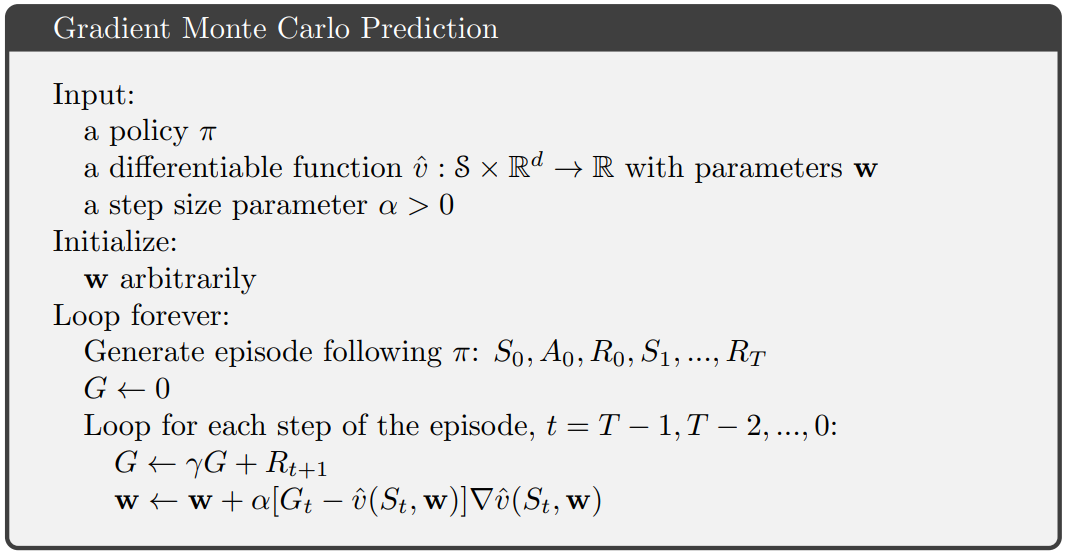
\includegraphics[width = \columnwidth]{figures/DeepReinforcementLearning2/GDMonteCarlo.png}
\end{figure}

\subsection{Deep Q-Learning}
\begin{figure}[!h]
    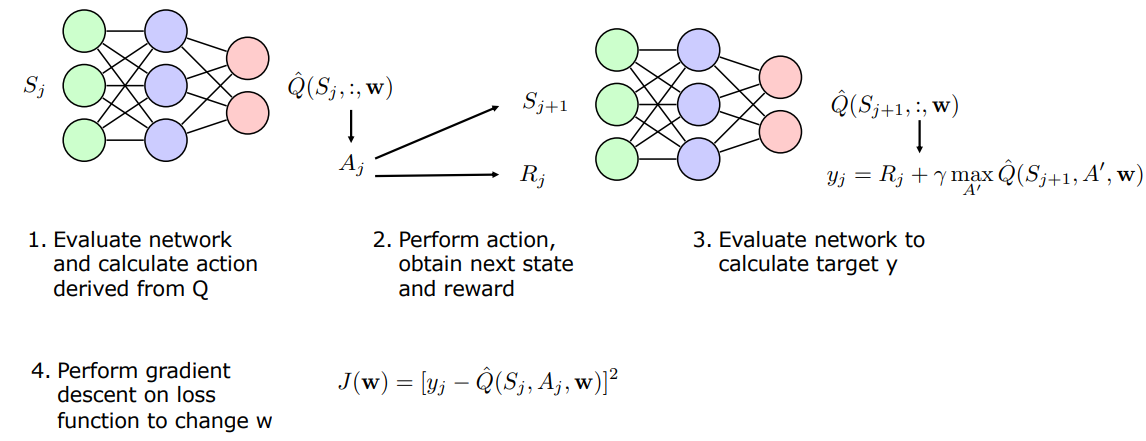
\includegraphics[width = \columnwidth]{figures/DeepReinforcementLearning2/BasicDeepQLearning.png}
\end{figure}
Use a neural network to approximate the Q-Function.
As multiple actions are needed to evaluate, multiple passes through the network are required.

A better approach is to use a neural network with inputs \(s\) to calculate the action-value function for all the actions simultaneously.
The output is a vector with a different q values for a given state.


\subsubsection{Problem: Moving Target}
\begin{itemize}
    \item As the calculation of the target function also depends on \textbf{w}, it will also be changed after a gradient step
    \item The target moves with every update to \textbf{w} while we are trying to approximate it.
    \item It is better to let the target remain stable, for this, another set of weights \(\boldsymbol{w}^-\) can be used that are updated after a few step.
\end{itemize}

\subsection{Experience Replay}
\begin{itemize}
    \item It is not efficient to update the network after one step
    \item Futhermore, a sample should be used more than once, similar to supervised learning, where we go over the data set multiple times
\end{itemize}
The \textbf{experience} at each time step is stored into a data set
\begin{align*}
    e_t &= (s_t, a_t, r_t, s_{t+1})\\
    D &= e_1, \dots, e_N
\end{align*}
\begin{itemize}
    \item A fixed size buffer is used that overwrites the oldest experience
    \item Training data then \textbf{sampled} from the data set
\end{itemize}
\begin{figure}[!h]
    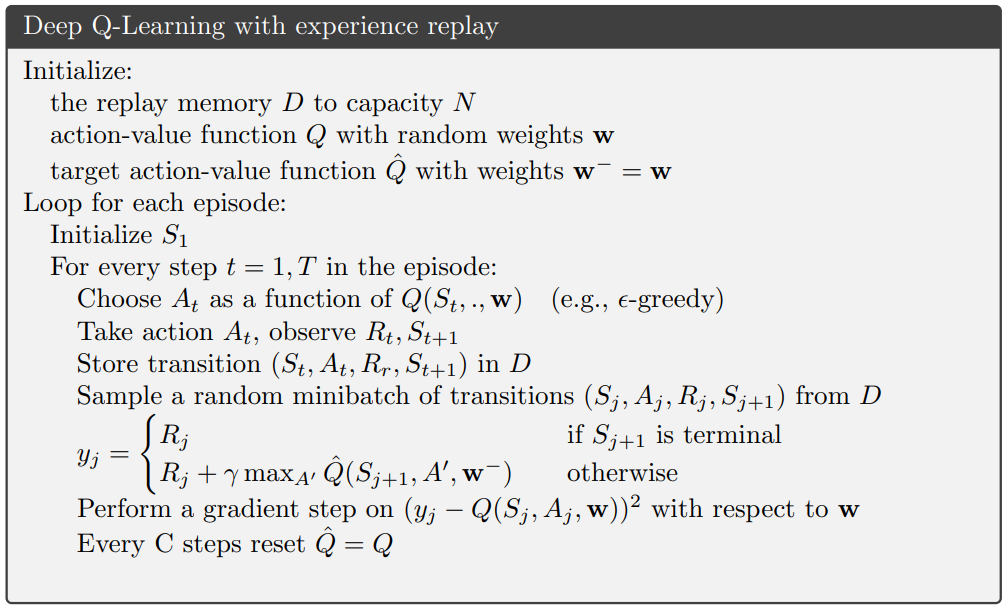
\includegraphics[width = \columnwidth]{figures/DeepReinforcementLearning2/DeepQLearningExperienceReplay.png}
\end{figure}

\subsection{Optimizing Deep Q-Learning}
Training for Deep Q-Learning is often difficult; several further concepts have been developed to make training easier:
\begin{itemize}
    \item Prioritized Experience Replay
    \item Double Q-Learning
    \item Dueling Networks
    \item Multi-step bootstrap targets
    \item Distributional DQN
    \item Noisy DQN
    \item Options of target weights update
\end{itemize}

\subsection{Policy Based Methods}
\begin{itemize}
    \item So far, all methods have been \textit{action-value methods}
    \item Policies were only calculated from those action-value estimates (using GPI)
    \item We now turn to methods that directly learn a parmetrized policy
    \[
    \pi(a|s,\boldsymbol{\theta}) = Pr\left\{A_t = a|S_t = s,\boldsymbol{\theta}_t = \boldsymbol{\theta}\right\}
    \]
    where \(\boldsymbol{\theta}\) are the parameters (weights) of the function that approximates the policy
\end{itemize}
\subsubsection*{Goal: Maximize Performance}
We want to change the weights, so that the return is maximized.
There are different algorithms to do that:
\begin{itemize}
    \item "Hill Climbing"
    \item Gradient Ascent
\end{itemize}

\subsubsection*{Policy Optimization with Hill Climbing}
Idea:
\begin{enumerate}
    \item Initialize weights for the function approximation arbitrarily
    \item Calculate the return \(G\) of an episode using the weights
    \item Change the weights slightly (add random noise)
    \item Calculate the return \(G\) using the new weights
    \item If return is larger: keep the new weights, decrease noise
    \item Otherwise: restore old weights, increase noise
    \item Continue with step 3
\end{enumerate}

\subsubsection{Why Policy-Based Methods}
\begin{itemize}
    \item While the goal of RL has been defiend is to maximize return \dots
    \item \dots we are not intrested in the actual value function, but
    \item \dots the \textbf{goal is to find the policy}
    \item Policy-based methods can learn true \textbf{stochastic policies}, this is different from epsilon greedy methods which add randomness just exploration
    \item Aliased states: States that look similar (same observation) but are actually different are difficult to handle with deterministic policies
    \item Finding the optimal action in values-based methods is difficult for continuous action spaces
\end{itemize}

\subsection{Policy Gradient Methods}
\begin{itemize}
    \item \textbf{Policy-based methods:} Search for optimal policy
    \item \textbf{Policy gradient methods:} Use \textbf{gradient ascent} to find the best parameters (Requires the approximation function to be differentiable)
    \[
    \boldsymbol{\theta}_{t+1} = \boldsymbol{\theta} + \alpha \widehat{\nabla J(\boldsymbol{\theta})}
    \]
    where
    \[
    \widehat{\nabla J(\boldsymbol{\theta})}
    \]
    is a stochastic estimate of the gradient of the performance measure.
\end{itemize}

\subsubsection*{Constrains for the policy}
The policy should be a probability function over the different actions and must use exploration, therefor:
\begin{itemize}
    \item The probability of any action should be greater than 0:
    \[
    \pi(a|s,\boldsymbol{\theta}) > 0, \text{for all } a \in A,s \in S
    \]
    \item The sum of all probabilities must be 1:
    \[
    \sum_{a}^{}\pi(a|s,\boldsymbol{\theta}) = 1, \text{for all } s \in S
    \]
    \item Use action-preferences and softmax:
    \[
    h(s,a,\mathbf{\theta})\in\mathbb{R} \qquad \pi(a|s,\boldsymbol{\theta}) = \frac{e^{h(s,a,\boldsymbol{\theta})}}{\sum_{b}^{e^{h(s,b,\boldsymbol{\theta})}}}
    \]
\end{itemize}

\subsubsection*{Episodic case}
\begin{itemize}
    \item Goal: optimize the total return from a (particular) state
    \[
    J(\boldsymbol{\theta}) = v_{\pi\boldsymbol{\theta}}(s_0)
    \]
    \item Problem: v depends on action selection and state distribution
    \item Policy gradient theorem:
    \[
    \nabla J({\boldsymbol{\theta}})\propto \sum_{s}^{}\mu(s)\sum_{a}^{}q_\pi(s,a)\nabla\pi(a|s,\boldsymbol{\theta})
    \]
\end{itemize}

\subsubsection*{REINFORCE: Monte Carlo Policy Gradient}
\begin{itemize}
    \item Update the weights according to:
    \begin{align*}
        \boldsymbol{\theta}_{t+1} &= \boldsymbol{\theta} + \alpha G_t\frac{\nabla\pi(A_t|S_t,\boldsymbol{\theta})}{\pi(A_t|S_t,\boldsymbol{\theta})}\\
        &= \boldsymbol{\theta} + \alpha G_t\nabla ln\pi(A_t|S_t, \boldsymbol{\theta})
    \end{align*}
    \item The second line can be derived from
    \[
    \nabla ln(f(x)) = \frac{\nabla f(x)}{f(x)}
    \]
    \item This is gradient \textbf{ascent}, as we want to maximize the return
\end{itemize}
\subsubsection*{How policy gradient works}
\begin{itemize}
    \item After the episode is complete, the policy gradient algorithm will look at each state and consider the selected action.
    \item If the return G was to high, it will make the action more likely
    \item If the return was low, it will reduce the probability
\end{itemize}

\subsubsection*{Problems with REINFORCE}
Policy Gradient is Noisy!
\begin{itemize}
    \item Gradient should be over millions episodes or trajectories (truncated episodes)
    \item But we typically only use one trajectory
    \item We should generate a number of trajectories, and calculate the trajectory from them 
    \item We can then also reduce noise by calculating the mean and standard deviation of the samples by reward normalization, this is called batch normalization
\end{itemize}

\subsubsection*{Baseline}
A "trick" for faster convergence and less variance is to subtract a baseline from the q values, where the baseline can be any function that does not depend on the action
\[
\nabla J({\boldsymbol{\theta}})\propto \sum_{s}^{}\mu(s)\sum_{a}^{}(q_\pi(s,a)-b(s))\nabla\pi(a|s,\boldsymbol{\theta})
\]
\[
    \boldsymbol{\theta}_{t+1} = \boldsymbol{\theta} + \alpha (G_t-b(S_t))\frac{\nabla\pi(A_t|S_t,\boldsymbol{\theta})}{\pi(A_t|S_t,\boldsymbol{\theta})}
\]
\begin{itemize}
    \item A natural choice for b, is to estimate a state value
    \[
    \hat{v}(S_t,\boldsymbol{w})
    \]
    \item where the weights would also be learned using the Monte-Carlo method
    \item The function is not dependent on the policy parametrization, so the gradient remains the same
    \item The difference between q and v is also called the \textit{advantage} function:
    \[
    q(s,a) - v(s)
    \]
\end{itemize}

\subsubsection*{Why does this baseline help?}
\begin{itemize}
    \item The current policy is used to sample actions, while the policy is also update from observations from the same actions.
    \item This creates an exploration-exploitation dilemma
    \item With a value baseline, the aggressiveness of the updates is reduced
\end{itemize}
\subsubsection{Summary Policy Gradient Methods}
Advantages:
\begin{itemize}
    \item Often better convergence properties
    \item Effective in high dimensional or continuous action spaces
    \item Can learn stochastic policies
\end{itemize}
Disadvantages:
\begin{itemize}
    \item Typically converge to local rather than global optimum
    \item Evaluating a policy can be inefficient and high variance
\end{itemize}
\subsubsection*{More on policy gradient Methods}
\begin{itemize}
    \item This was the \textit{vanilla} policy gradient method
    \item There are variations regarding the update and the sampling that make the methods more stable and faster to converge
    \item These are the Trust Region Policy Optimization (TRPO) and the Proximal Policy Gradient (PPO) methods
\end{itemize}

\subsection{Actor-Critic Methods}
1-step Policy Gradient Method with Critic
\begin{itemize}
    \item We would like to implement a 1-step (or n-step) method like TD(0) for the policy
    \item However, we then need a \textbf{value} function, so we can replace the full return in REINFORCE with the 1-step return:
    \begin{align*}
        \boldsymbol{\theta}_{t+1} &= \boldsymbol{\theta}_t + \alpha(R_t + \gamma\hat{v}(S_{t+1},\boldsymbol{w})-\hat{v}(S_t,\boldsymbol{w}))\nabla \text{ln}\pi(A_t|S_t,\boldsymbol{\theta}_t)\\
        &= \boldsymbol{\theta}_t + \alpha\delta_t\nabla \text{ln}\pi(A_t|S_t,\boldsymbol{\theta}_t)
    \end{align*}
    \item The policy is called the \textit{actor}, the value function the \textit{critic}
    \item The value function approximation can be calculated as in deep Q-Learning
\end{itemize}
\begin{figure}[!h]
    \centering
    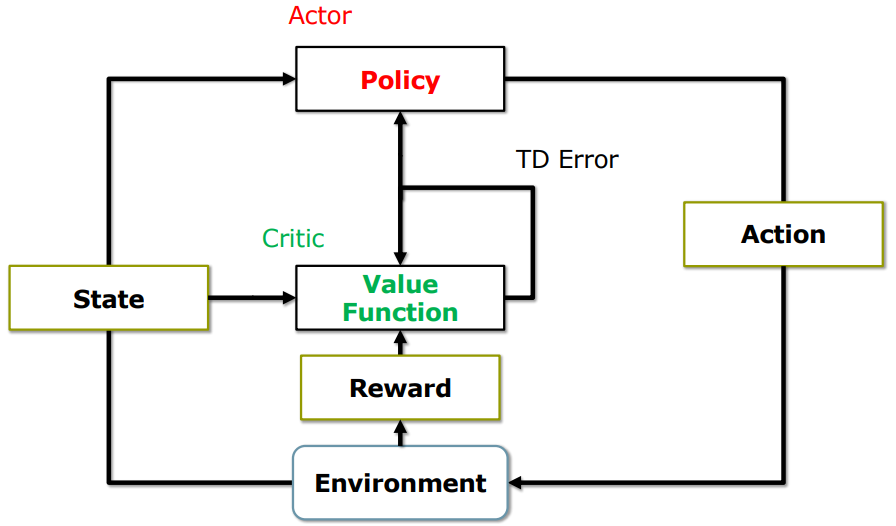
\includegraphics[width = \columnwidth]{figures/DeepReinforcementLearning2/ActorCritic.png}
\end{figure}

\subsection{Overview: Value and Policy based Methods}
Value Based:
\begin{itemize}
    \item Learnt Value Function
    \item Implicit Policy (e.g. epsilon greedy)
\end{itemize}
Policy Based:
\begin{itemize}
    \item No Value Function
    \item Learnt Policy
\end{itemize}
Actor-Critic
\begin{itemize}
    \item Learnt Value Function
    \item Learnt Policy
\end{itemize}

\subsubsection*{Example: How to play tennis?}
Policy based(REINFORCE):
\begin{itemize}
    \item Play matches
    \item Think about the matches that you won and lost, and do more of the actions you did in the won matches and less of those in the lost matches
\end{itemize}
Value based
\begin{itemize}
    \item You guess what the score will be like (during the match) and select actions that maximize the score
    \item Guesses get better, resulting in better performance
    \item but guesses can be wrong(biased, prone to over or underestimate)
\end{itemize}
Actor-Critic based:
\begin{itemize}
    \item Combine both approaches
    \item Actor Critic methods are more stable than value-based agents and need fewer samples than policy-based approaches
\end{itemize}
\subsubsection*{Different Actor-Critic/Policy Gradient Methods}
There are different choices for the value of \(\psi\) in the expression for the gradient:
\[
\psi \nabla_{\boldsymbol{\theta}} \text{ln}\pi(A_t|S_t,\boldsymbol{\theta})
\]
\begin{table}[!h]
    \begin{tabular}{lr}
    \(\psi = G\)    &  Return from episode\\
    \(\psi = Q(A_t,S_t)\)     &  Action-value function\\
    \(\psi = A(A_t,S_t)\)     &  Advantage function\\
    \(\psi = r_t + V(S')-V(S)\)     & TD(0) residual
    \end{tabular}
\end{table}